\chapter{Implementação}
\label{ch::impl}

%\section{Introdução}
%\label{sec::impl:intro}

A implementação do projeto \theapp~será detalhada no presente Capítulo, com particular foco nos seguintes pontos:

\begin{itemize}[nosep]
	\item Requisitos funcionais do projeto;
	\item Estrutura do código e o fluxo do mesmo;
	\item Detalhes de implementação e desafios encontrados.
\end{itemize}


\section{Funcionalidades e Requisitos}
\label{sec::impl:requisitos}

O projeto \theapp~segue uma lista de \textbf{funcionalidades} a implementar baseados nos objetivos do projeto (Secção \ref{sec::intro:objetivos}), em específico:

\begin{itemize}
    \item Renderização de funções implícitas com uso de \textit{ray marching};
    \item Suporte a dois motores de cálculo:
    \begin{enumerate}[nosep]
        \item Por \textit{software} (i.e. os cálculos são efetuados pela \ac{CPU});
        \item Aceleração por \textit{hardware} (com uso da \ac{GPU});
    \end{enumerate}
    \item Suporte a ficheiros externos contendo as funções implícitas a renderizar.
\end{itemize}

Foram ainda considerados os seguintes \textbf{requisitos} adicionais:
\begin{itemize}
    \item Abrir qualquer ficheiro \verb|.function| dinamicamente por um meio gráfico (\ac{GUI});
    \item Capacidade de personalizar a cor da superfície implícita;
    \item Apresentar as \ac{fps} alcançadas pelo programa para análise dos resultados.
\end{itemize}


\section{Lógica e Estruturação}
\label{sec::impl:estrutura}

A aplicação é composta por uma coletânea de classes, as quais comunicam entre si de forma a gerir a representação das funções implícitas em memória. O fluxo da aplicação é representado pela Figura \ref{fig::fluxo}.

A classe principal do programa é a \textbf{\ac{SISM}}. Esta é encarregue pelo ciclo de renderização pela gestão dos \textit{shaders}, carregados aquando do arranque do programa pelo \textit{Shader Loader}.

%\begin{figure}[!hbp]
%	\centering
%	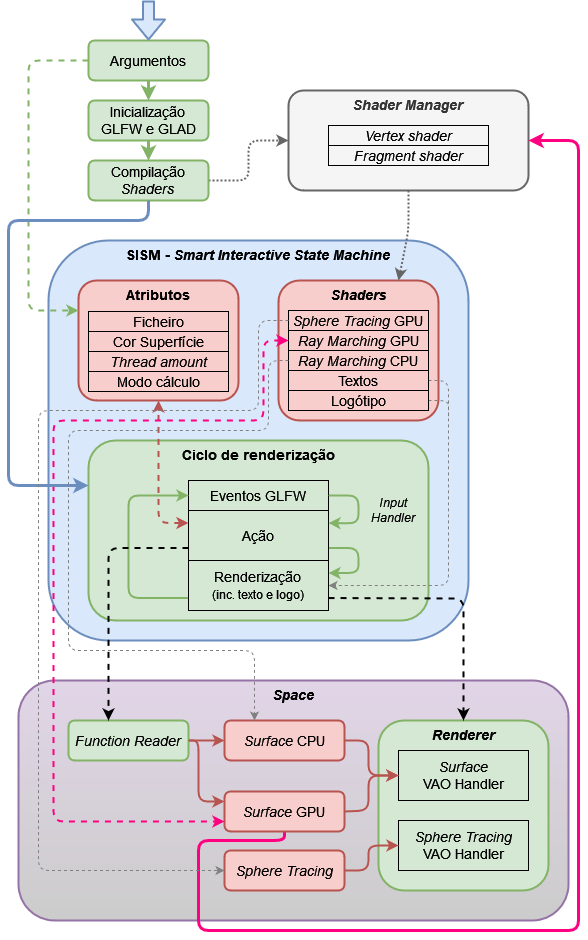
\includegraphics[width=.8\textwidth]{fluxo}
%	\caption[Fluxo de execução da \theapp]{Representação esquemática do fluxo da \theapp.}
%	\label{fig::fluxo}
%\end{figure}



\subsection{Parâmetros de arranque}
\label{ssec::impl:estrutura:start}

O programa disponibiliza uma coleção de argumentos que podem ser passados pela linha de comandos (ou terminal) para alterar o seu comportamento:

\begin{itemize}
    \item \verb|--width| ou \verb|-W|:\\
    Modifica a largura da janela de renderização, em pixeis.\\
    \textit{Default}: 600.\\
    Exemplo: \verb|-W 1000| inicia o programa com uma largura de 1000 pixeis.
    
    \item \verb|--height| ou \verb|-H|:\\
    Modifica a altura da janela de renderização, em pixeis.\\
    \textit{Default}: 600.\\
    Exemplo: \verb|-H 1000| inicia o programa com uma altura de 1000 pixeis.

    \item \verb|--render| ou \verb|-r|:\\
    Define qual o motor de renderização a que o programa recorre.\\
    Existem três modos implementados:
    \begin{itemize}[nosep]
        \item \verb|CPU|: motor de renderização por \textit{software} com uso do algoritmo naïve \textit{ray marching};
        \item \verb|GPU|: motor de renderização por aceleração de \textit{hardware} com uso do algoritmo naïve \textit{ray marching};
        \item \verb|SPHERES|: permite ao motor de renderização usar uma demonstração do algoritmo \textit{sphere tracing};
    \end{itemize}
	\textit{Default}: \verb|GPU|.
    
    \item \verb|--threads| ou \verb|-t|:\\
    Indica o número de \textit{threads} que devem ser usadas pelo motor de renderização por \textit{software}.\\
    \textit{Default}: metade do número de núcleos lógicos disponibilizados pela \ac{CPU}.\\
    Só é considerada caso o modo de renderização seja \verb|CPU|. Se o número especificado for superior ao \textit{default}, o utilizador é alertado para a possibilidade de problemas de \textit{performance} no seu sistema.\\
    Exemplo: \verb|-t 6| inicia o programa com seis \textit{threads} prontas a serem usadas.
\end{itemize}

Está ainda disponível o comando de ajuda descrito como o argumento \verb|--help| ou \verb|-h|, nesta situação o programa emite a informação descrevendo os argumentos disponíveis e em seguida este sai do programa.

O processamento destes argumentos define o estado dos seguintes atributos da \ac{SISM}:
\begin{itemize}[nosep]
    \item Motor de renderização;
    \item Resolução da janela.
\end{itemize}


\subsection{\textit{Shader Manager}}
\label{ssec::impl:estrutura:shaders}

Este passo de arranque do programa só é feito caso a inicialização das bibliotecas/\textit{frameworks} GLFW e \ac{GLAD} seja corretamente efetuada.

Os \textit{shaders} são carregados pelo \textit{Shader Manager}, o qual é instanciado para cada um dos cinco programas (num total de dez \textit{shaders} a compilar, cada um com o seu respetivo \textit{vertex} e \textit{fragment shaders}):

\begin{enumerate}[nosep]
	\item Motor de renderização por \acs{CPU};
	\item Motor de renderização acelerado por \textit{hardware} (\acs{GPU});
	\item Motor de teste de \textit{sphere tracing} (por \acs{GPU});
	\item Logótipo;
	\item Textos.
\end{enumerate}

Anteriormente à compilação dos mesmos é efetuada uma \textbf{verificação automática} dos \textit{shaders}. Caso algum esteja em falta, o programa é capaz de criar o respetivo \textit{shader} predefinido e procede à sua compilação.

Assim que todos os \textit{shaders} sejam corretamente compilados, é gerada uma janela com a dimensão definida pelo atributo do \ac{SISM}. É esperado em caso de sucesso o seguinte \textit{output}:

\begin{verbatim}
Lauching CalcGL...
    Setting global variables...     
    Setting relevant directories... [OK]
    Initializing GLFW and GLAD... [OK]
    Auto-checking shaders... (corrected 0 shaders) [OK]
    Loading shaders... [OK]
    Loading text renderer... [OK]
    Loading logo... [OK]
Done.
\end{verbatim}


\section{Motores de renderização}
\label{sec::impl:motor}

Dos três modos de renderização disponibilizados, dois são motores propriamente ditos (por \textit{software} e acelerado por \textit{hardware}) e o terceiro é um modo de demonstração de \textit{sphere tracing}. Nos dois primeiros, as funções são obtidas por ficheiros externos com a extensão \verb|*.function|. É obrigatório que as funções estejam escritas segundo a sintaxe da linguagem \ac{GLSL}.


\subsection{Cálculo por \textit{Software}}
\label{ssec::impl:motor:cpu}

Este motor de renderização pode executar em várias \textit{threads}, onde cada uma processa um conjunto de linhas contíguas do plano de visualização. As funções são processadas pela biblioteca \textit{CParse} e o algoritmo de \textit{ray marching} utilizado é o \textbf{naïve com \textit{bisection}}.


\subsection{Aceleração por \textit{hardware}}
\label{ssec::impl:motor:gpu}

O motor de renderização acelerado por \textit{hardware} faz a \textbf{injeção de funções} no \textit{fragment shader} utilizado por este modo. Uma vez que o \textit{Shader Manager} pode compilar programas a qualquer momento, as funções lidas do ficheiro \verb|*.function| são injetadas num local predeterminado do \textit{fragment shader} padrão e um novo programa é compilado com este novo \textit{shader}, sendo o anterior descartado.

A parte do \textit{fragment shader} modificado é o seguinte:

\begin{minted}[linenos]{glsl}
// Defines a implicit function
float evalImplicitFunc(vec3 point) {
    float x = point.x;
    float y = point.y;
    float z = point.z;
    float prod = 1.f;

    // <gamma conditions>

    return prod;
}
\end{minted}

As funções lidas são multiplicadas a fim de formar uma Superfície $\Pi$ com um fator de \textit{blending} $r = 0$. A sua injeção é feita no local do comentário indicado por \verb|<gamma conditions>|. Por exemplo, caso o ficheiro defina três esferas:

\begin{eqnarray*}
	x^2 + y^2 + z^2 - 1 = 0 \\
	(x-2)^2 + (y-1)^2 + z^2 - 1 = 0 \\
	(x-1)^2 + (y-2)^2 + (z-2)^2 - 1 = 0
\end{eqnarray*}

O \textit{fragment shader} será recompilado com as seguintes linhas de código no lugar de \verb|<gamma conditions>|.

\begin{minted}[linenos,firstnumber=8]{glsl}
prod *= pow(x, 2.) + pow(y, 2.) + pow(z, 2.) - 1.;
prod *= pow(x-2., 2.) + pow(y-1., 2.) + pow(z, 2.) - 1.;
prod *= pow(x-1., 2.) + pow(y-2., 2.) + pow(z-2., 2.) - 1.;
\end{minted}

Este modo \textbf{não implementa \textit{bisection}} devido a uma limitação ao nível da \acs{GPU}.

Sendo unidades de cálculo muito especializadas, as \acsp{GPU} não contemplam instruções de \textit{interrupt}, cuja consequência é a impossibilidade de parar os programas por si executados (conjunto de \textit{shaders}) uma vez iniciados. Os \textit{shaders} podem entrar em ciclos infinitos, os quais levariam ao total bloqueio de todo o sistema operativo por indisponibilidade da \acs{GPU}. Desta forma, o sistema operativo monitoriza o tempo de cada execução da \acs{GPU} e, caso ultrapasse um determinado \textit{threshold} por si definido, é-lhe feito um \textit{reset}.

Por este motivo, a implementação de \textit{bisection} levou a este fenómeno de \textit{reset} da \acs{GPU}, pelo que foi excluído do algoritmo final implementado no \textit{fragment shader}.

Há ainda a notar que este motor não verifica as funções fornecidas nos ficheiros \verb|*.function| uma vez que não se enquadrava no objetivo principal do projeto.


\subsection{Demonstração de \textit{Sphere Tracing}}
\label{ssec::impl:motor:sphere}

O modo de demonstração de \textit{sphere tracing} distingue-se dos demais uma vez que implementa diretamente no seu \textit{fragment shader} as superfícies a serem renderizadas, estando então as respetivas \acfp{SDF} presentes diretamente no código. Outras funções implícitas não podem ser renderizadas, servindo então para mero efeito ilustrativo deste algoritmo de \textit{ray marching}.


%\section{Conclusões}
%\label{sec::impl:conc}
